\section{Наклонная волоконная брэгговская решётка}
Чтобы понять физику наклонных волокон удобно рассмотреть спектры коэффицентов 
пропускания и отражения пары идентичных решёток наклонённые относительно друг друга на $ 10 $ градусов.
Можно выделить два важных случая: cлучай нормальной волоконной брэгговской решётки у которой только один сильный резонанс. К примеру провал в спектре пропускания соответствует условию Брэгга для периода решётки в этом волокне и тот же резонанся появляется как одиничный пик в спектре отражения. Длина волна $ \lambda_{B} $ соответсвующая брэгговскому резонансу самая большая так эффективный показатель преломления для одной моды направленной вдоль сердцевины самый большой.

В дополнение к брэгговскому резонансу, спектр наклонной решётки Брэгга иммеет большое количество сопутствующих резонансов, но только в спектре пропускания. Эти резонансы возникают из-за взаимодействия мод друг с другом.Оболочечные моды не видны в спектре отражения так как исчезают из-за потерь в оболочке Когда решётка наклонена, самый существенный эффект это значительное усиление оболочечных мод за счёт основной.
Ближайший к брэгговскому резонанс обычно сильнее своего оболочечного соседа со коротковолновой стороны и называется "призрачной" модой так как по своим свойства она очень похожа на брегговский резонанс, но
является суперпозицией нескольких оболочечных мод малого порядка. В спектре пропускания наклонной решётки есть значение около $ 1530 $ нм где непрерывость в оболочечной моде теряется после которой (в коротко
волновую сторону) наблюдается резкое убываение резонансных амплитуд. Этот эффект объясняется переходом от направленных оболочечных мод к оболочечным модам с потерями.







\begin{figure}[h]
	\centering
	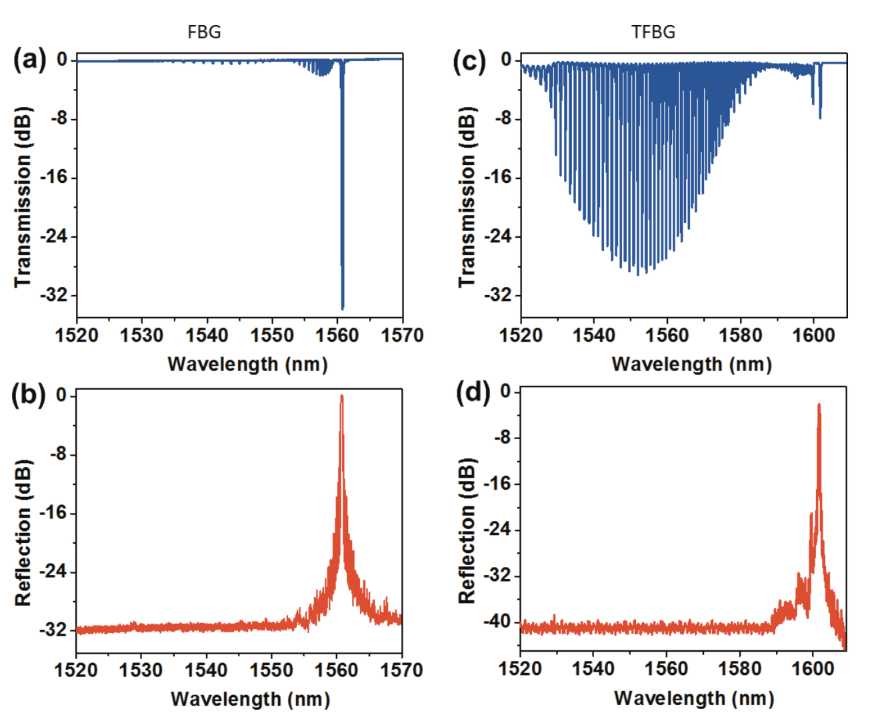
\includegraphics[width=0.7\linewidth]{screenshot001}
	\caption{}
	\label{fig:screenshot001}
\end{figure}


\par
Дифракция на решётке проходит эффективно тогда и только тогда удоволетворены два условия: закон сохранения импульса (иначе говоря фазы совпадают)


$$\beta_{i} \pm \beta_{G}=\beta_{j}$$ 

\begin{figure}
	\centering
	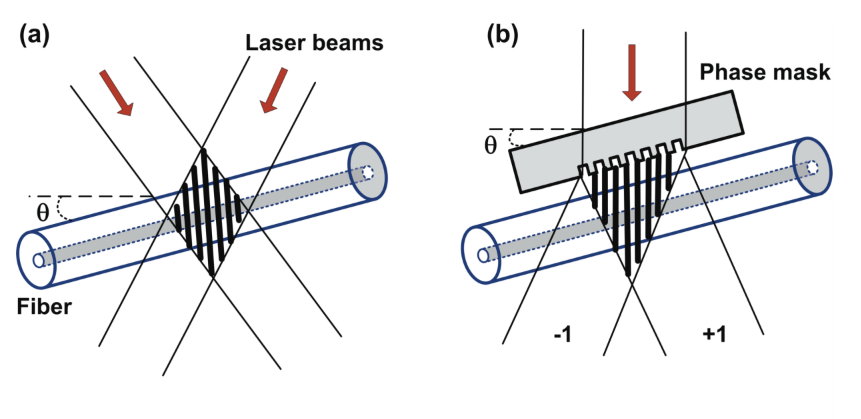
\includegraphics[width=0.7\linewidth]{screenshot005}
	\caption{}
	\label{fig:screenshot005}
\end{figure}


\begin{figure}[h]
	\centering
	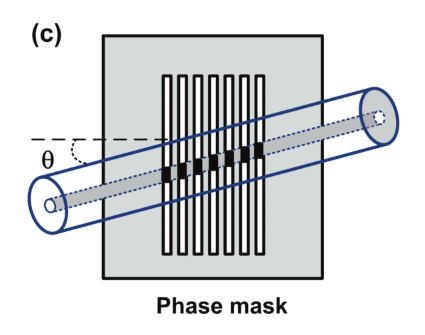
\includegraphics[width=0.4\linewidth]{screenshot004}
	\caption{}
	\label{fig:screenshot004}
\end{figure}

\subsection{Собственные оптические свойства наклонной решётки}

С увеличением угла наклона огибающа взаимодействующих резонансов смещается в коротковолновую сторону. Самая часто используемая и полезная конфигурация удобная для химических сенсоров это угол в 10 градусов так как эффективный коэффицент преломления её преобладающей оболочечной резонансной моды перекрывает очень важную область около значения $ 1.3 $.
\begin{figure}
	\centering
	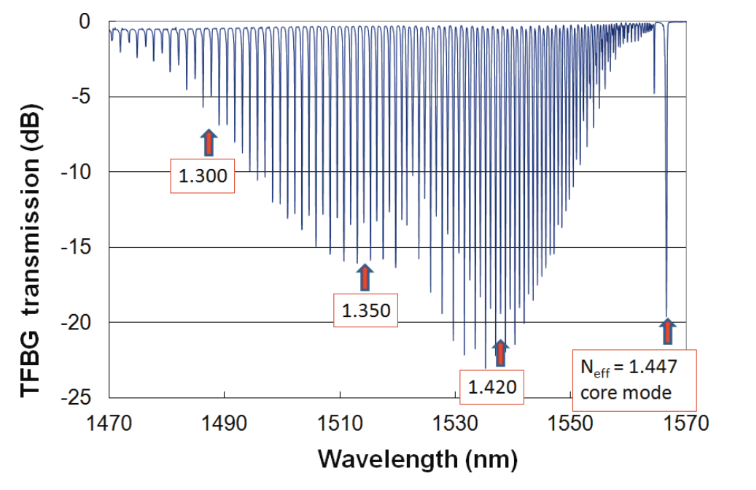
\includegraphics[width=0.7\linewidth]{screenshot006}
	\caption{}
	\label{fig:screenshot006}
\end{figure}


Очень сильные  резонансные взаимодействия (потеря пропускания около 20 $dB$ соответствующая захвату  $ 99\%   $ входного света оболочечной модой с определённой частотой) достигается с похожей шириной резонанса что и в нормальный решётке, примерно 0.1 нм для решётки длинной 1 см. Также возможно участить период решётки и тем самым расширить резонансы и даже сделать их полностью перекрывающимися получив гладкий пропускной фильтр. Абсолютные и относительные  амплитуды Брэгговского резонанса и призрачная мода значительно изменяются с углом наклона.

\par

Хотя брэгговсикй резонанс присутствует только в отражении в дальнейшем мы покажем, что отражающая оболочечная мода сенсора может быть имплементирована с помощью разных промежуточных сред для области сердцевина-оболочка. Другой опцией является использование наклонной решётки в отражающей конфигурации поставив рефлектор далельше от решётки так чтобы свет прошёл бы через наклонную решётку дважду и вернулся бы к источнику. В своём простейшем исполнении, хорошая щель обеспечит широкополостное отражение пары процентов падающего света достаточное для измерения пропускных резонансов оболочечной моды. Для более эффективного использования света, можно накрыть зеркальной прослойкой (золото или серебро) на последующей выемке для 100\% отражения падающего света. Другой вариант для отражателя может быть сделан и обычной прямой брэгговской решётки с подобранным спектром отражения так чтобы желанный волновой диапазон спектра наклонной решётки отражался как показано на рисунке.



\par 
Ещё одным важным параметром является поляризация света. Поляризация очень сильно влияет на спетра наклонной решётки


\subsection{Влияние угла наклона, длины и силы решётки}
 Для начала можно  переписать условие совпадения фаз в более удобной форме.
 Так для длины волны $ \lambda_{r} $ резонанся решётки между основной моды и другой обозначенной через $ r $
$$\lambda_{r}=\left(N_{\mathrm{eff}}^{\mathrm{core}}\left(\lambda_{r}\right)+N_{\mathrm{eff}}^{r}\left(\lambda_{r}\right)\right) \Lambda / \cos (\theta)$$

 Где $ \Lambda $ период интерференционных полос используемых] для создания решётки, $ \theta $ угол наклона плоскости решётки относительно плоскости поперечного сечения.
 $N_{\mathrm{eff}}^{\mathrm{core}}\left(\lambda_{r}\right)$ эффективный коэффицент преломления одной моды направленной через сердцевину на длине волны на которой наблюдается резонанся $ \lambda_{r} $ b $$N_{\mathrm{eff}}^{\mathrm{r}}\left(\lambda_{r}\right)$$ эффектиный коэффицент преломления моды $ r $ на той же длине волне. Важно учитывать дисперсию так как резонансы оболочечной моды возникают на сравнительно широком спектральном промежутке (Более 100 нм в случае угла наклона в 10 градусов).
 
\par
Cила решёточного резонанса (отражательная мощность $ R $) зависит от коэффицента перекрытия $ \kappa $ между 
падающей основной модой и той модой которая совпадает с ней по фазе.
Так для решётки длинной $ L $ Отражательная мощность выражается через




$$R=\tanh ^{2}(\kappa L)$$


$$\kappa=C \iint_{-\infty}^{\infty} \vec{E}_{\mathrm{core}}^{*} \cdot \vec{E}_{r} \Delta \mathrm{n}(\mathrm{x}, \mathrm{y}) \mathrm{d} \mathrm{xdy}$$


где $ С $ коэффицент пропорициональности связанный с нормировкой $ E_{core} $ и $ E_{r}$ и  $\Delta \mathrm{n}(\mathrm{x}, \mathrm{y})$ - функция описывающая возмущение коэффицента преломления из-зп присутствия решётки в поперечном сечении волокна.


Для большинства обычных решёток, и в частности, для решётки которая рассматривается в этой работе, возмущённая область показателя преломления для решётки ограничена сердцевиной и равна нулю в остальном пространстве. Поэтому бесконечные пределы в интеграле можно заменить на границу сердцевины.
Более того, входная мода линейно поляризована вдоль случайного направления
из-за цилиндрической симметрии задачи. Возмущение решётки имеет хорошо определённую ориентацию в пространстве которая нарушает симметрию волокна вдоль направления наклона (назовём эту плосткость плоскостью $yz$  с напрвелнием распространения вдоль $ z $). Поэтому, можно рассматривать отдельно два граничных случая: волна поляризованная вдоль $ x $  ($ S $-поляризация ) или $ y $ ($ P $-поляризация).Наконец, cкалярное произведение электрических полей в интеграле редуцируется на обычное произведение к умножению $ x $ или $ y $ поляризованных полей (в зависимотсти от входящей волны), так как $\Delta n(x , y)$ не является тензором для стёкл. Заметив, что интегрирование ведётся по $ xy $ срезу волокна, решёточное возмущение на области ингрирования является константой для обычной решётки но имеет более сложное поведение для наклонной решётки.

$$\Delta n(x, y)=\Delta n \cos ((4 \pi / \Lambda)(z \cos (\theta)+y \sin (\theta))$$

Для ясности картины отметим что когда входная мода поляризована вдоль $ x $
интеграл включает только $ x $ - компоненту оболочечной моды электрического поля (аналогично для $ y $ - поляризованной моды). Эти два случая можно рассматривать отдельно (а все остальные рассматривать как суперпозицию этих двух ортогональных состояний). В итоге, для заданного возмущения показателя преломления решётки, оболочечные моды для которых интеграл даёт сильное взаимодействие будут другими в зависимости от ориентированности полярзации входной моды относительно угла наклона (так как $ E_x $ и $ E_y $ компоненты поля для заданной оболочечной моды довольно отличаются)
 
\begin{figure}[h]
	\centering
	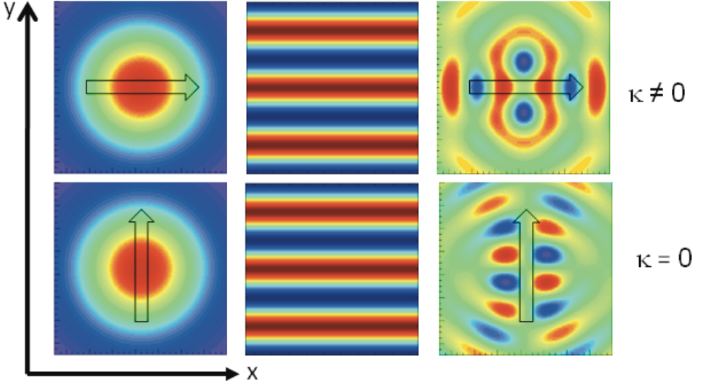
\includegraphics[width=0.7\linewidth]{screenshot008}
	\caption{}
	\label{fig:screenshot008}
\end{figure}

\subsection{Дисперсия плазмона}
Из-за полнового внутреннего отражения от границы сердцевина-оболочка и оболочка-внешняя граница всем соответствующие моды остаются локализованы. Это означает, что дисперсионные кривые мод оболочки лежат в области между световыми конусами, соответствующими внешней среде и материалу оболочки \ref{fig:screenshot012}. $ n_{exter} $ и $ n_{cladd} $  – показатели преломления внешней среды и оболочки соответственно. Дисперсионная кривая моды сердцевины, в свою очередь, проходит между световыми конусами оболочки и сердцевины. В реальной системе коэффициент преломления сердцевины   отличается от   на величину порядка. Поэтому дисперсию моды сердцевины можно аппроксимировать дисперсией волны в материале волокна (стекле), пренебрегая отличием между оболочкой и сердцевиной:где   – волновое число моды сердцевины.
Резонансное взаимодействие моды сердцевины с брэгговским зеркалом сводится к перебросу дисперсионной кривой на постоянную обратной решетки  , где   – период брэгговской решетки (рис 10). Частота, соответствующая пересечению полученной кривой с дисперсионной кривой моды, бегущей по сердцевине в обратном направлении, есть частота брэгговского отражения в моду сердцевины. На этой частоте наблюдается резкий минимум коэффициента прохождения . Сказанное означает, что волновое число   в 2 раза больше волнового числа моды сердцевины, испытывающей брэгговское отражение (условие Брэгга). Зная длину волны брэгговского резонанса, находим постоянную обратной решетки:
На более высоких частотах (меньших длинах волн) кривая последовательно пересекает различные моды оболочки, что соответствует системе провалов в спектре прохождения.



\begin{figure}[h]
	\centering
	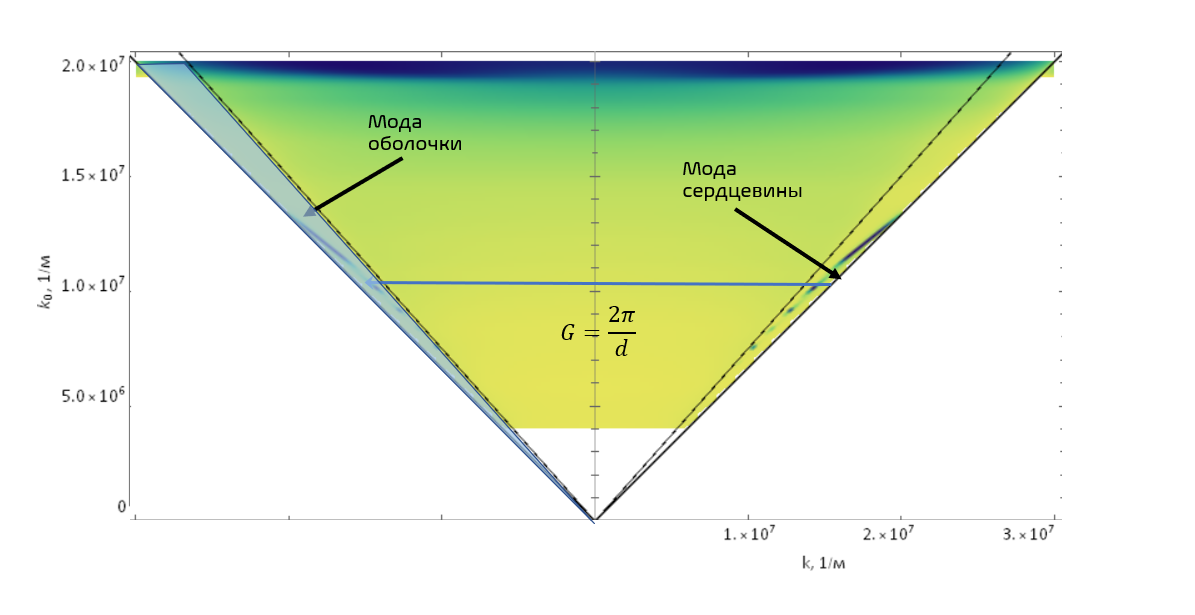
\includegraphics[width=0.9\linewidth]{screenshot012}
	\caption{}
	\label{fig:screenshot012}
\end{figure}



\subsection{Зависимость коэффицента пропускания от показателя преломления внешней среды}
 Во многих экспериментальных работах проводились опыты, где наклонную решётку с золотым напылением опускали в разные жидкости с разными коэффицентами преломления для измерения их рефрактометрической чувствиетительности. На рисунке \ref{fig:screenshot010} показаны измерения спектрального коэффицента пропускания для трёх разных показателей преломления. На графиках отчётливо видны области где амплитуда осцилляций значительно меньше чем в остальных областях и их сдвиг в зависимости от коэффицента преломления.
 Засекая длину волны при которой начинается такое поведение можно с очень высокой точностью измерять коэффицент преломления жидкостей.







 
 \begin{figure}[h]
 	\centering
 	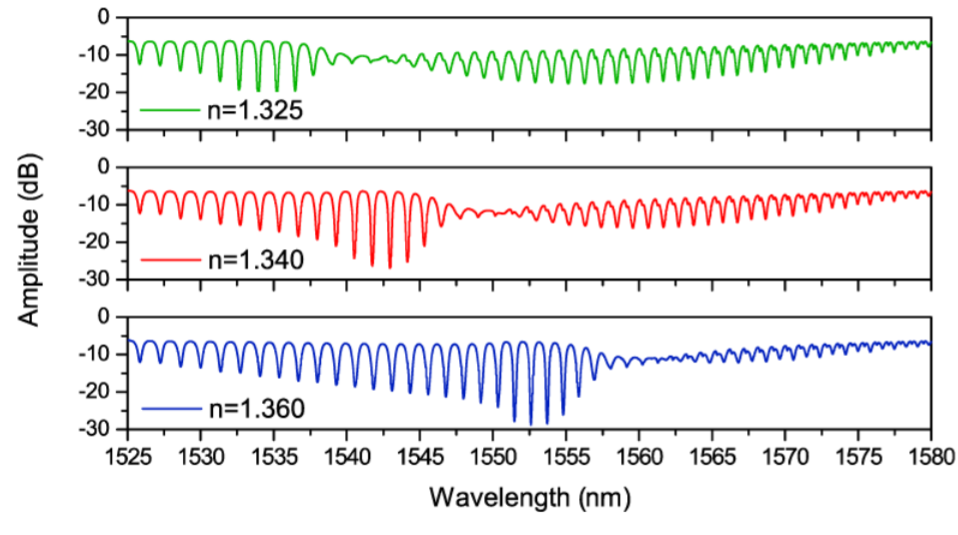
\includegraphics[width=0.7\linewidth]{screenshot010}
 	\caption{}
 	\label{fig:screenshot010}
 \end{figure}
 